%% LyX 2.4.4 created this file.  For more info, see https://www.lyx.org/.
%% Do not edit unless you really know what you are doing.
\documentclass[oneside,english]{book}
\usepackage[T1]{fontenc}
\usepackage[latin9]{inputenc}
\setcounter{secnumdepth}{3}
\setcounter{tocdepth}{3}
\usepackage{amsmath}
\usepackage{amsthm}
\usepackage{amssymb}
\usepackage{geometry}
\geometry{verbose,tmargin=1in,bmargin=1in,lmargin=1.5in,rmargin=1.5in}

\makeatletter

%%%%%%%%%%%%%%%%%%%%%%%%%%%%%% LyX specific LaTeX commands.
%% Because html converters don't know tabularnewline
\providecommand{\tabularnewline}{\\}

%%%%%%%%%%%%%%%%%%%%%%%%%%%%%% Textclass specific LaTeX commands.
\theoremstyle{definition}
\newtheorem{defn}{\protect\definitionname}
\theoremstyle{plain}
\newtheorem{thm}{\protect\theoremname}

%%%%%%%%%%%%%%%%%%%%%%%%%%%%%% User specified LaTeX commands.
\usepackage{hyperref}
\usepackage[usenames,dvipsnames]{xcolor} %adds additional color options
\hypersetup{colorlinks=true, urlcolor=Blue}%Blue

\usepackage{multicol}

\usepackage{tikz}
\usepackage{tikz-3dplot}

\usetikzlibrary{calc,arrows,shapes,backgrounds,matrix,shapes.geometric,fit,trees,positioning}

\usetikzlibrary{patterns}
\usetikzlibrary{plotmarks}
\usepackage{pgfplots}
\pgfplotsset{compat=newest}

\usepackage{calc}
\usepackage[nomessages]{fp}

\usepackage{datetime}
%\usepackage{subcaption}

%\usepackage{amsthm}

%%%%%commands
\newcommand{\mb}[1]{$\mathbb{#1}$}
\newcommand{\funct}[2]{$f\colon#1\rightarrow#2$}
% Added by lyx2lyx
\setlength{\parskip}{\smallskipamount}
\setlength{\parindent}{0pt}

\makeatother

\usepackage{babel}
\providecommand{\definitionname}{Definition}
\providecommand{\theoremname}{Theorem}

\begin{document}

\chapter{\label{chap:Homomorphisms-and-Isomorphisms}Homomorphisms and Isomorphisms}

Consider the two groups $\mathbb{Z}_{6}$ and $\mathbb{Z}_{2}\times\mathbb{Z}_{3}$
(under addition). $\mathbb{Z}_{6}=\{0,1,2,3,4,5\}$ and 
\[
\mathbb{Z}_{2}\times\mathbb{Z}_{3}=\{(0,0),(0,1),(0,2),(1,0),(1,1),(1,2)\}\mbox{.}
\]
These groups have the same number of elements, but as it turns out
they have much more in common. Pair the elements as follows:

\begin{table}[h]
\begin{centering}
\begin{tabular}{cccccc}
0 & 1 & 2 & 3 & 4 & 5\tabularnewline
$\downarrow$ & $\downarrow$ & $\downarrow$ & $\downarrow$ & $\downarrow$ & $\downarrow$\tabularnewline
(0,0) & (1,1) & (0,2) & (1,0) & (0,1) & (1,2)\tabularnewline
\end{tabular}
\par\end{centering}
\caption{\label{tab:iso-ex}The elements from $\mathbb{Z}_{6}$ are mapped
to $\mathbb{Z}_{2}\times\mathbb{Z}_{3}$. }
\end{table}
This map identifies the zero and identities of each group, $0\rightarrow(0,0)$
and $1\rightarrow(1,1)$ respectively. Note that in $\mathbb{Z}_{6}$,
$3+4=1\mod 6$ and in $\mathbb{Z}_{2}\times\mathbb{Z}_{3}$, $(1,0)+(0,1)=(1,1)$.
Our map identifies $1\rightarrow(1,1)$. Our map can be formulated
with $(3x+4y)\mod 6\rightarrow(x,y)$ is a function from $f\colon\mathbb{Z}_{6}\rightarrow\mathbb{Z}_{2}\times\mathbb{Z}_{3}$.

Though these groups appear quite different, this function shows that
their behavior is identical. We will call this function an \emph{isomorphism}
and two such groups \emph{isomorphic. }

\section{Functions}

We covered functions in MTH 335, but that was a while ago.
\begin{defn}
A \emph{function }(or \emph{mapping) }from sets $A$ to $B$\emph{,
$f\colon A\rightarrow B$,} is a rule that assigns each element in
$A$ to exactly one element in $B$.
\end{defn}
\begin{itemize}
\item $A$ is called the \emph{domain }of $f$. 

\begin{itemize}
\item $B$ is called the \emph{range }of $f$.\footnote{Also called the \emph{co-domain.}}
\item If $f(a)=b$ for some $a\in A$, then $b$ is called the\emph{ image
of $a$ under $f$.}
\item $\{b\colon b\in B\mbox{ and }f(a)=b\mbox{ for some }a\in A\}$ is
called the \emph{image of} $A$ \emph{under $f$}.
\end{itemize}
\item Functions are well defined. Meaning that an input is assigned to one
and only output. 
\end{itemize}
\begin{defn}
Let $f\colon A\rightarrow B$ and $g\colon B\rightarrow C$. The \emph{composition}
of $g\circ f$ is the mapping from $A$ to $C$ defined as follows:
$g\circ f(a)=g(f(a))$ for any $a\in A$.
\end{defn}
\begin{figure}
\begin{centering}
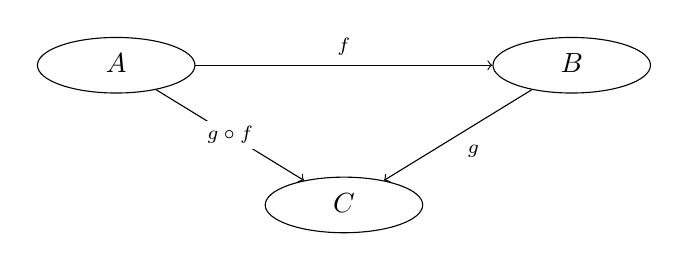
\begin{tikzpicture}[description/.style={fill=white,inner sep=2pt}]   
	\matrix (m)[matrix of math nodes,     
	row sep=3em,column sep=2.5em,     
	text height=1.5ex, text depth=0.25ex,     	nodes={ellipse,draw,minimum width=2cm},   	]
	{
		A && B \\     
		& C & 
		\\   };   
	\path[->,font=\scriptsize]   (m-1-1) edge node[auto] {$ f $} (m-1-3)   edge node[description] {$ g \circ f $} (m-2-2)   (m-1-3) edge node[auto] {$ g $} (m-2-2); \end{tikzpicture}
\par\end{centering}
\caption{Composition of functions $f$ and $g$.}
\end{figure}

\begin{defn}
A function, \funct{A}{B}, is called \emph{one-to-one}\footnote{Also called an \emph{injective function}}
if $f(a_{1})=f(a_{2})$ implies that $a_{1}=a_{2}$.

A function \funct{A}{B} is \emph{onto }if for every $b\in B$ there
is an $a\in A$ such that $f(a)=b$.
\end{defn}
\begin{figure}[h]
\hfill%
\begin{minipage}[t]{0.33\textwidth}%
 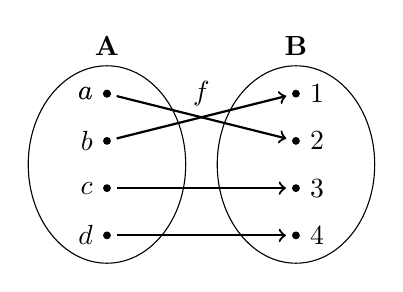
\begin{tikzpicture}[scale=.6,ele/.style={fill=black,circle,minimum width=.8pt,inner sep=1pt},every fit/.style={ellipse,draw,inner sep=-2pt}]   
	\node[label=center:$\textbf{A}$] (a0) at (0,5) {};
	\node[ele,label=left:$a$] (a1) at (0,4) {};
	\node[ele,label=left:$a$] (a1) at (0,4) {};       
	\node[ele,label=left:$b$] (a2) at (0,3) {};       
	\node[ele,label=left:$c$] (a3) at (0,2) {};   
	\node[ele,label=left:$d$] (a4) at (0,1) {};
	\node[label=center:$\textbf{B}$] (b0) at (4,5) {};	
	\node[ele,,label=right:$1$] (b1) at (4,4) {};   
	\node[ele,,label=right:$2$] (b2) at (4,3) {};   
	\node[ele,,label=right:$3$] (b3) at (4,2) {};   
	\node[ele,,label=right:$4$] (b4) at (4,1) {};
	\node[draw,fit= (a1) (a2) (a3) (a4),minimum width=2cm] {};
	\node[label=center:$f$] 
(f1) at (2,4) {};
	 
	\node[draw,fit= (b1) (b2) (b3) (b4),minimum width=2cm] {};     
	
	\draw[->,thick,shorten <=2pt,shorten >=2pt] (a1) -- (b2);   
	\draw[->,thick,shorten <=2pt,shorten >=2] (a2) -- (b1);   
	\draw[->,thick,shorten <=2pt,shorten >=2] (a3) -- (b3);   
	\draw[->,thick,shorten <=2pt,shorten >=2] (a4) -- (b4);  
\end{tikzpicture}\caption{}{\funct{A}{B} is  one-to-one and onto.}%
\end{minipage}\hfill%
\begin{minipage}[t]{0.33\textwidth}%
\begin{center}
 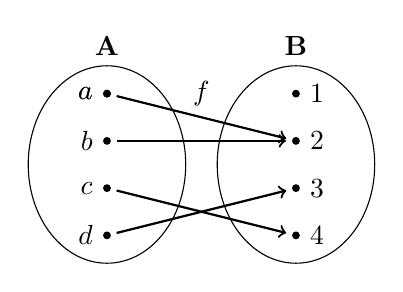
\begin{tikzpicture}[scale=.6,ele/.style={fill=black,circle,minimum width=.8pt,inner sep=1pt},every fit/.style={ellipse,draw,inner sep=-2pt}]   
	\node[label=center:$\textbf{A}$] (a0) at (0,5) {};
	\node[ele,label=left:$a$] (a1) at (0,4) {};
	\node[ele,label=left:$a$] (a1) at (0,4) {};       
	\node[ele,label=left:$b$] (a2) at (0,3) {};       
	\node[ele,label=left:$c$] (a3) at (0,2) {};   
	\node[ele,label=left:$d$] (a4) at (0,1) {};
	\node[label=center:$\textbf{B}$] (b0) at (4,5) {};	
	\node[ele,,label=right:$1$] (b1) at (4,4) {};   
	\node[ele,,label=right:$2$] (b2) at (4,3) {};   
	\node[ele,,label=right:$3$] (b3) at (4,2) {};   
	\node[ele,,label=right:$4$] (b4) at (4,1) {};
	\node[draw,fit= (a1) (a2) (a3) (a4),minimum width=2cm] {};
	\node[label=center:$f$] 
(f1) at (2,4) {};
	 
	\node[draw,fit= (b1) (b2) (b3) (b4),minimum width=2cm] {};     
	
	\draw[->,thick,shorten <=2pt,shorten >=2pt] (a1) -- (b2);   
	\draw[->,thick,shorten <=2pt,shorten >=2] (a2) -- (b2);   
	\draw[->,thick,shorten <=2pt,shorten >=2] (a3) -- (b4);   
	\draw[->,thick,shorten <=2pt,shorten >=2] (a4) -- (b3);  
\end{tikzpicture}\caption{}{\funct{A}{B} is not one-to-one and is not onto.}
\par\end{center}%
\end{minipage}\hfill%
\begin{minipage}[t]{0.33\textwidth}%
\begin{center}
 \begin{tikzpicture}[scale=.6,ele/.style={fill=black,circle,minimum width=.8pt,inner sep=1pt},every fit/.style={ellipse,draw,inner sep=-2pt}]   
	\node[label=center:$\textbf{A}$] (a0) at (0,5) {};
	\node[ele,label=left:$a$] (a1) at (0,4) {};
	\node[ele,label=left:$a$] (a1) at (0,4) {};       
	\node[ele,label=left:$b$] (a2) at (0,3) {};       
	\node[ele,label=left:$c$] (a3) at (0,2) {};   
	\node[ele,label=left:$d$] (a4) at (0,1) {};
	\node[label=center:$\textbf{B}$] (b0) at (4,5) {};	
	%\node[ele,,label=right:$1$] (b1) at (4,4) {};   
	\node[ele,,label=right:$2$] (b2) at (4,3) {};   
	\node[ele,,label=right:$3$] (b3) at (4,2) {};   
	\node[ele,,label=right:$4$] (b4) at (4,1) {};
	\node[draw,fit= (a1) (a2) (a3) (a4),minimum width=2cm] {};
	\node[label=center:$f$] 
(f1) at (2,4) {};
	 
	\node[draw,fit= (b1) (b2) (b3) (b4),minimum width=2cm] {};     
	
	\draw[->,thick,shorten <=2pt,shorten >=2pt] (a1) -- (b2);   
	\draw[->,thick,shorten <=2pt,shorten >=2] (a2) -- (b2);   
	\draw[->,thick,shorten <=2pt,shorten >=2] (a3) -- (b4);   
	\draw[->,thick,shorten <=2pt,shorten >=2] (a4) -- (b3);  
\end{tikzpicture}\caption{}{\funct{A}{B} is onto but not one-to-one.}
\par\end{center}%
\end{minipage}\hfill
\end{figure}


\section{Homomorphism}
\begin{defn}
\label{def: A-(ring)-homomorphism,}A (\emph{ring}) \emph{homomorphism},\emph{
$f$}, from a ring $R$ to a ring $S$ is a function $f\colon R\rightarrow S$
that preserves the two ring operations:
\[
f(a+b)=f(a)+f(b)\mbox{ and }f(ab)=f(a)f(b)
\]
for $a,b\in R$. 
\end{defn}
\begin{thm}
\textbf{\emph{\label{thm:Properties-of-Ring}Properties of Ring Homomorphisms.}}\textbf{
}Let $f$ be a ring homomorphism from rings $R$ to $S$, and let
$A$ be a subring of $R$.
\end{thm}
\begin{enumerate}
\item $f(0_{R})=0_{s}$.
\item \emph{$f(-a)=-f(a)$ for every $a\in R$.}
\item \emph{$f(a-b)=f(a)-f(b)$ for every $a,b\in R$.}
\item \emph{For any $a\in R$ and any positive integer $n$, $f(nr)=nf(r)$
and $f(r^{n})=f(r)^{n}$.}
\item \emph{If $R$ is commutative then $f(R)$ is commutative.}
\item \emph{$f(A)=\{f(a)\colon a\in A\}$ is a subring of $S$.}
\item \emph{If $R$ has unity $1_{R}$, $S\neq\{0\}$, and $f$ is onto}

\begin{enumerate}
\item \emph{then $f(1_{R})$ is the unity of $S$.}
\item \emph{if $aa^{-1}=1_{R}$ for any $a,a^{-1}\in R$, then $f(a)f(a^{-1})=1_{S}$
and $f(a)^{-1}=f(a^{-1})$.}
\end{enumerate}
\end{enumerate}

\section{Isomorphisms}
\begin{defn}
A \emph{ring} \emph{isomorphism} from a ring $R$ to a ring $S$ is
a function that is one-to-one and onto.
\end{defn}

\begin{defn}
If there exists a ring isomorphism $f\colon R\rightarrow S$ then
$R$ and $S$ are said to be \emph{isomorphic}.  
\end{defn}
Showing that two rings are isomorphic usually requires finding an
isomorphism between the, and this can be tricky at times. However
looking at the properties from theorem \ref{thm:Properties-of-Ring}
can serve as a guide.
\end{document}
